% !TEX program = xelatex
\documentclass[12pt,a4paper]{article}

% =================== PACKAGES ===================
\usepackage[T1]{fontenc}
\usepackage{geometry}
\usepackage{graphicx}
\usepackage{hyperref}
\usepackage{enumitem}
\usepackage{titlesec}
\usepackage{fancyhdr}
\usepackage{booktabs}
\usepackage{array}
\usepackage{tabularx}
\usepackage{longtable}
\usepackage{setspace}
\usepackage[final,nopatch=footnote]{microtype}
\usepackage{newtxtext}
\usepackage{parskip}
\usepackage[nottoc]{tocbibind}
\usepackage{tikz}
\usetikzlibrary{arrows.meta, positioning, shapes.geometric, backgrounds, calc, fit, matrix}
\usepackage{caption}
\captionsetup{font=small, labelfont=bf, margin=0.5cm}
\usepackage{float}
\usepackage{xcolor}
\usepackage{pdflscape}
\usepackage{ragged2e}
\usepackage{makecell}
\graphicspath{{fig/}}

% =================== PAGE LAYOUT ===================
\geometry{
  top=1in,
  bottom=1in,
  left=1.05in,
  right=1.05in,
  headheight=14pt,
  headsep=18pt
}
\setstretch{1.12}
\setlength{\emergencystretch}{3em}

% =================== COLOURS ===================
\definecolor{lkblue}{HTML}{1F5B8F}
\definecolor{lkcyan}{HTML}{E9F4FB}
\definecolor{lkgreen}{HTML}{2E7D32}
\definecolor{lkorange}{HTML}{C46A1A}
\definecolor{lkpurple}{HTML}{6A4C93}
\definecolor{lkgray}{HTML}{F4F6F8}
\definecolor{darkgray}{HTML}{333333}

% =================== HEADER / FOOTER ===================
\pagestyle{fancy}
\fancyhf{}
\fancyhead[L]{\small IK2015 Enterprise Architecture}
\fancyhead[R]{\small Seminar 5: Zachman Framework \& Relational Data Model}
\fancyfoot[C]{\thepage}
\renewcommand{\headrulewidth}{0.4pt}

% =================== SECTION FORMATTING ===================
\titleformat{\section}[hang]{\Large\bfseries\color{darkgray}}{\thesection}{1em}{}
\titleformat{\subsection}[hang]{\large\bfseries\color{darkgray}}{\thesubsection}{1em}{}
\titleformat{\subsubsection}[hang]{\normalsize\bfseries\color{darkgray}}{\thesubsubsection}{1em}{}
\titlespacing*{\section}{0pt}{12pt}{6pt}
\titlespacing*{\subsection}{0pt}{10pt}{4pt}
\titlespacing*{\subsubsection}{0pt}{8pt}{2pt}

% =================== HYPERLINK SETUP ===================
\hypersetup{
  colorlinks=true,
  linkcolor=black,
  citecolor=black,
  urlcolor=lkblue,
  pageanchor=false
}

% =================== TABLE HELPERS ===================
\newcolumntype{Y}{>{\RaggedRight\arraybackslash}X}
\newcolumntype{P}[1]{>{\RaggedRight\arraybackslash}p{#1}}
\renewcommand{\arraystretch}{1.22}
\newcommand{\pk}[1]{\underline{#1}}
\newcommand{\fk}{\textsuperscript{FK}}
\newcommand{\pkfk}{\textsuperscript{PK, FK}}
\newcommand{\nullable}{\textsuperscript{nullable}}

% =================== TITLE AREA ===================
\title{}
\author{}
\date{}

\begin{document}

% ---- Custom Title Page ----
\thispagestyle{empty}
\vspace*{1.8cm}

\begin{center}
  {\normalsize Jiangxi University of Finance and Economics} \\[2.1cm]

  {\LARGE\bfseries Zachman Framework and Relational Data Model} \\[0.15cm]
  {\LARGE\bfseries Report} \\[1.0cm]

  {\Large Luckin Coffee Inc.} \\[0.25cm]
  {\normalsize\itshape A Technology-Driven New Retail Coffee Enterprise} \\[2.0cm]

  {\normalsize IK2015: Enterprise Architecture and Database Programming} \\[0.2cm]
  {\normalsize Seminar 5} \\[2.2cm]

  {\normalsize\textbf{Group 4}} \\[0.45cm]
  {\normalsize
    Zhe-Kai Yang~(Krust),\quad
    Shi-Hang Chen~(Sean),\quad
    Wei-Yu Cai~(Nosta), \\[0.2cm]
    Huan-Wen Chen~(Evan),\quad
    Yuan-Yong Liao~(Foreve)
  } \\[1.8cm]

  {\normalsize \today}
\end{center}

\newpage
\hypersetup{pageanchor=true}
\setcounter{page}{1}
\pagenumbering{arabic}
\pagestyle{fancy}

% =================== BASIC INFORMATION ===================
\section{Report Basic Information}

\begin{table}[H]
\centering
\caption{Basic information of the Seminar 5 report.}
\begin{tabularx}{\textwidth}{P{4.25cm}Y}
\toprule
\textbf{Item} & \textbf{Information} \\
\midrule
Selected enterprise / business & Luckin Coffee Inc.; mobile-first coffee retail, pickup, delivery, partnership-store operation, and packaged coffee business. \\
Course and seminar & IK2015 Enterprise Architecture and Database Programming; Seminar 5. \\
Group number & Group 4. \\
Group members & \parbox[t]{\hsize}{\raggedright Zhe-Kai Yang~(Krust), Shi-Hang Chen~(Sean), Wei-Yu Cai~(Nosta),\\ Huan-Wen Chen~(Evan), Yuan-Yong Liao~(Foreve).} \\
Main deliverable & A Row 1 Scope description of the Zachman Framework for Luckin Coffee and a relational data model transformed from the Seminar 4 conceptual model. \\
\bottomrule
\end{tabularx}
\end{table}

This report follows the Seminar 5 instruction sheet. It first fills in the first row of the Zachman Framework for the selected case-study business, and then transforms the conceptual model developed in Seminar 4 into a relational data model. The transformation identifies relations, primary keys, foreign keys, bridge tables, and integrity rules that make the conceptual model implementable in a database.

% =================== ZACHMAN FRAMEWORK ROW 1 ===================
\section{Zachman Framework: Row 1 Scope}

The Zachman Framework is a classification scheme for enterprise architecture. It organizes architectural descriptions by two dimensions: stakeholder perspectives and basic interrogatives. In this report, only Row 1 is required. Row 1 is the \textbf{Scope} or \textbf{Contextual} perspective of the planner. It does not describe detailed system implementation; instead, it lists the high-level business things, processes, locations, organizations, events, and goals that define the enterprise boundary.

For Luckin Coffee, the Row 1 view is useful because the company combines digital ordering, physical store fulfilment, standardized recipes, supply resources, and performance feedback. The following table describes this scope across the six Zachman columns.

\begin{landscape}
\begin{table}[p]
\centering
\caption{Zachman Framework Row 1 Scope for Luckin Coffee Inc.}
\footnotesize
\renewcommand{\arraystretch}{1.12}
\begin{tabularx}{\linewidth}{>{\raggedright\arraybackslash\bfseries}p{2.15cm} *{6}{>{\raggedright\arraybackslash}X}}
\toprule
& \textbf{DATA} \newline (What?) & \textbf{FUNCTION} \newline (How?) & \textbf{NETWORK} \newline (Where?) & \textbf{PEOPLE} \newline (Who?) & \textbf{TIME} \newline (When?) & \textbf{MOTIVATION} \newline (Why?) \\
\midrule
SCOPE \newline (Contextual) \newline \textit{Planner}
& \begin{itemize}[leftmargin=*, nosep, label=-]
    \item Customers and members
    \item Digital channels
    \item Orders and order items
    \item Products and recipes
    \item Stores and staff
    \item Raw materials and suppliers
    \item Delivery partners
    \item Operational KPIs
  \end{itemize}
& \begin{itemize}[leftmargin=*, nosep, label=-]
    \item Attract and register customers
    \item Publish campaigns and coupons
    \item Accept mobile orders and payments
    \item Prepare pickup and delivery tasks
    \item Manage recipes and products
    \item Replenish store materials
    \item Monitor service and financial results
  \end{itemize}
& \begin{itemize}[leftmargin=*, nosep, label=-]
    \item Mobile app and mini-program
    \item Cloud ordering platform
    \item Headquarters planning units
    \item Self-operated and partner stores
    \item City retail locations
    \item Supplier origins and warehouses
    \item Delivery service areas
  \end{itemize}
& \begin{itemize}[leftmargin=*, nosep, label=-]
    \item Digital-native customers
    \item Members and coupon users
    \item Store managers and baristas
    \item Product and recipe teams
    \item Corporate planners
    \item Franchise or partner-store operators
    \item Material suppliers and delivery riders
  \end{itemize}
& \begin{itemize}[leftmargin=*, nosep, label=-]
    \item App sessions and campaign periods
    \item Order date and order time
    \item Real-time queue and preparation status
    \item Daily store operating hours
    \item Morning and lunch peak demand
    \item Weekly replenishment cycles
    \item Recipe-version effective dates
  \end{itemize}
& \begin{itemize}[leftmargin=*, nosep, label=-]
    \item Mobile-first new retail strategy
    \item Fast and standardized fulfilment
    \item Affordable premium positioning
    \item Customer lifetime value growth
    \item Product innovation and margin control
    \item Supply reliability
    \item Data-driven operating decisions
  \end{itemize} \\
\bottomrule
\end{tabularx}
\end{table}
\end{landscape}

This Row 1 scope clarifies what must remain connected when the architecture becomes more detailed. For example, the data column identifies the objects that later become database tables, while the function and time columns explain why order status, campaign validity, recipe versions, and replenishment timing must be represented explicitly.

% =================== CONCEPTUAL MODEL BASIS ===================
\section{Conceptual Model Used as the Source}

The relational data model below is transformed from the Seminar 4 conceptual model for Luckin Coffee. The conceptual model described Luckin as an integrated retail platform with demand-side, fulfilment-side, product-side, and resource-side objects. Its main business objects were Customer, Membership Account, Digital Channel, Promotion Campaign, Digital Order, Order Item, Product, Recipe Standard, Raw Material, Supplier, Store, Store Staff, Fulfilment Task, Delivery Partner, and Performance Result.

The conceptual relationships used for transformation are summarized as follows:
\begin{itemize}[leftmargin=1.3em]
  \item \textbf{Demand relationships}: customers use digital channels, customers own membership accounts, members place digital orders, and promotions are distributed to members and applied to orders.
  \item \textbf{Fulfilment relationships}: digital orders contain order items and create fulfilment tasks; fulfilment tasks are executed by stores and may involve delivery partners.
  \item \textbf{Product and resource relationships}: order items refer to products; products have recipe standards; recipes consume raw materials; suppliers provide materials; stores hold materials as inventory.
  \item \textbf{Analytical feedback}: performance results are derived from operational tables such as orders, fulfilment tasks, stores, campaigns, and delivery partners. Because these are calculated KPIs, they are implemented as reporting queries or views rather than as one base transaction table in the core schema.
\end{itemize}

% =================== RELATIONAL DATA MODEL ===================
\section{Relational Data Model Design}

The relational model applies standard mapping rules. Each major conceptual object becomes a relation. One-to-many relationships are represented by placing the primary key of the parent relation as a foreign key in the child relation. Many-to-many relationships are resolved using bridge relations with composite primary keys. The model also includes basic domain constraints, such as non-negative monetary values, valid status values, campaign date ranges, and recipe effective dates.

\subsection{Relations, Primary Keys, and Foreign Keys}

In the following table, underlined attributes are primary-key attributes. Attributes marked with FK reference another relation. Composite keys are shown by underlining more than one attribute in the same relation.

\scriptsize
\begin{longtable}{P{3.45cm}P{12.0cm}}
\caption{Relational data model transformed from the conceptual model.}\\
\toprule
\textbf{Relation} & \textbf{Attributes} \\
\midrule
\endfirsthead
\toprule
\textbf{Relation} & \textbf{Attributes} \\
\midrule
\endhead
\midrule
\multicolumn{2}{r}{\textit{Continued on next page}}\\
\endfoot
\bottomrule
\endlastfoot
Customers & \pk{CustomerId}, Segment, City, AgeBand \\
MembershipAccounts & \pk{MemberId}, CustomerId\fk~(Unique), PointsBalance, CouponValue, MemberTier, ActivityStatus \\
DigitalChannels & \pk{ChannelId}, ChannelType, AccessDevice, AppVersion \\
PromotionCampaigns & \pk{CampaignId}, CampaignType, TargetSegment, StartDate, EndDate, SubsidyAmount \\
MemberCampaigns & \pk{MemberId}\pkfk, \pk{CampaignId}\pkfk, ReceivedDate, UsedStatus \\
DigitalOrders & \pk{OrderId}, MemberId\fk, ChannelId\fk, PaymentMethod, QueueStatus, GrossOrderAmount, CampaignDiscountAmount, ItemDiscountAmount, ActualDeliveryFee, NetPayableAmount, OrderDate, OrderTime \\
OrderCampaigns & \pk{OrderId}\pkfk, MemberId\fk, \pk{CampaignId}\pkfk, AppliedAmount \\
Products & \pk{ProductId}, ProductName, Category, Season, GrossMargin, CurrentStandardCost \\
OrderItems & \pk{OrderId}\pkfk, \pk{ItemNr}, ProductId\fk, Quantity, Customization, LineDiscountAmount, UnitItemPrice \\
DeliveryPartners & \pk{PartnerId}, PartnerName, PartnerType, ServiceArea, StandardDeliveryFee, ComplaintRate \\
Stores & \pk{StoreId}, StoreName, OwnershipType, CityTier, LocationType, Revenue, LaborCost \\
FulfilmentTasks & \pk{TaskId}, OrderId\fk, StoreId\fk, PartnerId\fk\nullable, TaskType, PrepTime, WaitingTime, CompletionRate, Status \\
StoreStaff & \pk{StaffId}, StoreId\fk, StaffName, StaffRole, TrainingStatus, WorkingHours, LaborCost, Productivity \\
Suppliers & \pk{SupplierId}, SupplierName, SupplierType, LeadTime \\
RawMaterials & \pk{MaterialId}, SupplierId\fk, MaterialName, MaterialType, Origin, BatchStatus, InventoryValue \\
StoreMaterials & \pk{StoreId}\pkfk, \pk{MaterialId}\pkfk, StockLevel, StockoutRate \\
RecipeStandards & \pk{RecipeId}, ProductId\fk, RecipeVersion, SopStatus, RecipeStandardCost, DefectRate, EffectiveFrom, EffectiveTo \\
RecipeMaterials & \pk{RecipeId}\pkfk, \pk{MaterialId}\pkfk, DosageAmount, DosageUnit \\
\end{longtable}
\normalsize

\subsection{Foreign-Key Structure}

\begin{table}[H]
\centering
\caption{Main foreign-key dependencies in the relational data model.}
\footnotesize
\begin{tabularx}{\textwidth}{P{3.35cm}P{3.45cm}Y}
\toprule
\textbf{Foreign key in relation} & \textbf{References} & \textbf{Meaning} \\
\midrule
\makecell[l]{MembershipAccounts\\CustomerId} & \makecell[l]{Customers\\CustomerId} & One customer owns one membership account; the unique constraint prevents duplicate membership accounts for the same customer. \\
\makecell[l]{DigitalOrders\\MemberId} & \makecell[l]{MembershipAccounts\\MemberId} & A member can place many digital orders. \\
\makecell[l]{DigitalOrders\\ChannelId} & \makecell[l]{DigitalChannels\\ChannelId} & Each order is placed through one recorded digital channel. \\
\makecell[l]{MemberCampaigns\\MemberId} & \makecell[l]{MembershipAccounts\\MemberId} & A member can receive many campaigns. \\
\makecell[l]{MemberCampaigns\\CampaignId} & \makecell[l]{PromotionCampaigns\\CampaignId} & A campaign can be distributed to many members. \\
\makecell[l]{OrderCampaigns\\OrderId, MemberId} & \makecell[l]{DigitalOrders\\OrderId, MemberId} & A campaign usage is attached to a specific order and the member who placed it. \\
\makecell[l]{OrderCampaigns\\MemberId, CampaignId} & \makecell[l]{MemberCampaigns\\MemberId, CampaignId} & An order can only apply a campaign that was issued to that member. \\
\makecell[l]{OrderItems\\OrderId} & \makecell[l]{DigitalOrders\\OrderId} & One order can contain multiple product lines. \\
\makecell[l]{OrderItems\\ProductId} & \makecell[l]{Products\\ProductId} & Each order line sells one product. \\
\makecell[l]{FulfilmentTasks\\OrderId} & \makecell[l]{DigitalOrders\\OrderId} & One order may create preparation, pickup, delivery, or exception tasks. \\
\makecell[l]{FulfilmentTasks\\StoreId} & \makecell[l]{Stores\\StoreId} & Each fulfilment task is handled by one store. \\
\makecell[l]{FulfilmentTasks\\PartnerId} & \makecell[l]{DeliveryPartners\\PartnerId} & Delivery tasks may involve a delivery partner; pickup tasks may leave this value null. \\
\makecell[l]{StoreStaff\\StoreId} & \makecell[l]{Stores\\StoreId} & One store employs many staff members. \\
\makecell[l]{RawMaterials\\SupplierId} & \makecell[l]{Suppliers\\SupplierId} & One supplier can provide many materials. \\
\makecell[l]{StoreMaterials\\StoreId, MaterialId} & \makecell[l]{Stores\\StoreId;\\RawMaterials\\MaterialId} & Store inventory is represented as a bridge between stores and materials. \\
\makecell[l]{RecipeStandards\\ProductId} & \makecell[l]{Products\\ProductId} & A product can have multiple recipe versions. \\
\makecell[l]{RecipeMaterials\\RecipeId, MaterialId} & \makecell[l]{RecipeStandards\\RecipeId;\\RawMaterials\\MaterialId} & Recipe ingredients are represented as a bridge between recipes and materials. \\
\bottomrule
\end{tabularx}
\end{table}

\subsection{Mapping Logic from Conceptual Model to Relations}

\begin{table}[H]
\centering
\caption{Conceptual-to-relational mapping decisions.}
\small
\begin{tabularx}{\textwidth}{P{4.0cm}P{3.2cm}Y}
\toprule
\textbf{Conceptual element} & \textbf{Relational result} & \textbf{Reasoning} \\
\midrule
Customer and Membership Account & Customers; MembershipAccounts & These objects are separated because demographic segmentation and membership benefits have different attributes. The CustomerId foreign key in MembershipAccounts is unique, representing a one-to-one relationship. \\
Digital Channel and Digital Order & DigitalChannels; DigitalOrders & Channel information is stored once and referenced by orders. This avoids repeating app, mini-program, device, and version data in every order record. \\
Promotion Campaign issued to members & MemberCampaigns & The member-campaign relationship is many-to-many, so a bridge relation records which member received which campaign and whether it was used. \\
Promotion Campaign applied to orders & OrderCampaigns & A second bridge relation records actual campaign use on orders and the discount amount applied. Including MemberId keeps campaign use consistent with member campaign distribution. \\
Order and Order Item & DigitalOrders; OrderItems & Order-level fields such as payment method, queue status, and net amount are separated from product-line fields such as quantity, customization, discount, and unit price. \\
Product and Recipe Standard & Products; RecipeStandards & Product catalogue information is separated from recipe versions, SOP status, standard cost, and effective dates. This supports controlled product changes over time. \\
Recipe Standard and Raw Material & RecipeMaterials & Recipes and materials are many-to-many. The bridge relation records dosage amount and dosage unit for each ingredient. \\
Store and Raw Material & StoreMaterials & Stores hold many materials, and the same material can be stocked by many stores. The bridge relation records local stock level and stockout rate. \\
Order fulfilment and delivery & FulfilmentTasks; DeliveryPartners & Fulfilment work is separated from the purchase event, making preparation time, waiting time, completion rate, and delivery complaints measurable. \\
Performance Result & Reporting views or queries & KPIs such as average order value, campaign redemption rate, store utilization, and stockout rate are derived from operational relations rather than stored as a separate base transaction table. \\
\bottomrule
\end{tabularx}
\end{table}

The model also uses integrity constraints beyond simple key definitions. For example, order amounts must be non-negative, net payable amount equals gross amount minus campaign and item discounts plus actual delivery fee, campaign start date cannot be later than campaign end date, stock level cannot be negative, and recipe effective dates must be ordered correctly. The SQL implementation also uses triggers to ensure that a campaign applied to an order is valid for that order date and does not exceed the campaign subsidy amount.

% =================== SCHEMA DIAGRAMS ===================
\section{Relational Data Model Diagrams}

The relational data model is shown in two diagrams to keep the schema readable on A4 paper. The first diagram focuses on customer demand, digital orders, campaign use, and fulfilment. The second diagram focuses on products, recipes, materials, store inventory, and suppliers. Together, the two diagrams represent the same complete relational model listed in the relation table above.

\newgeometry{margin=1cm}
\begin{landscape}
\thispagestyle{empty}
\begin{figure}[p]
\centering
\begin{minipage}{26cm}
\centering
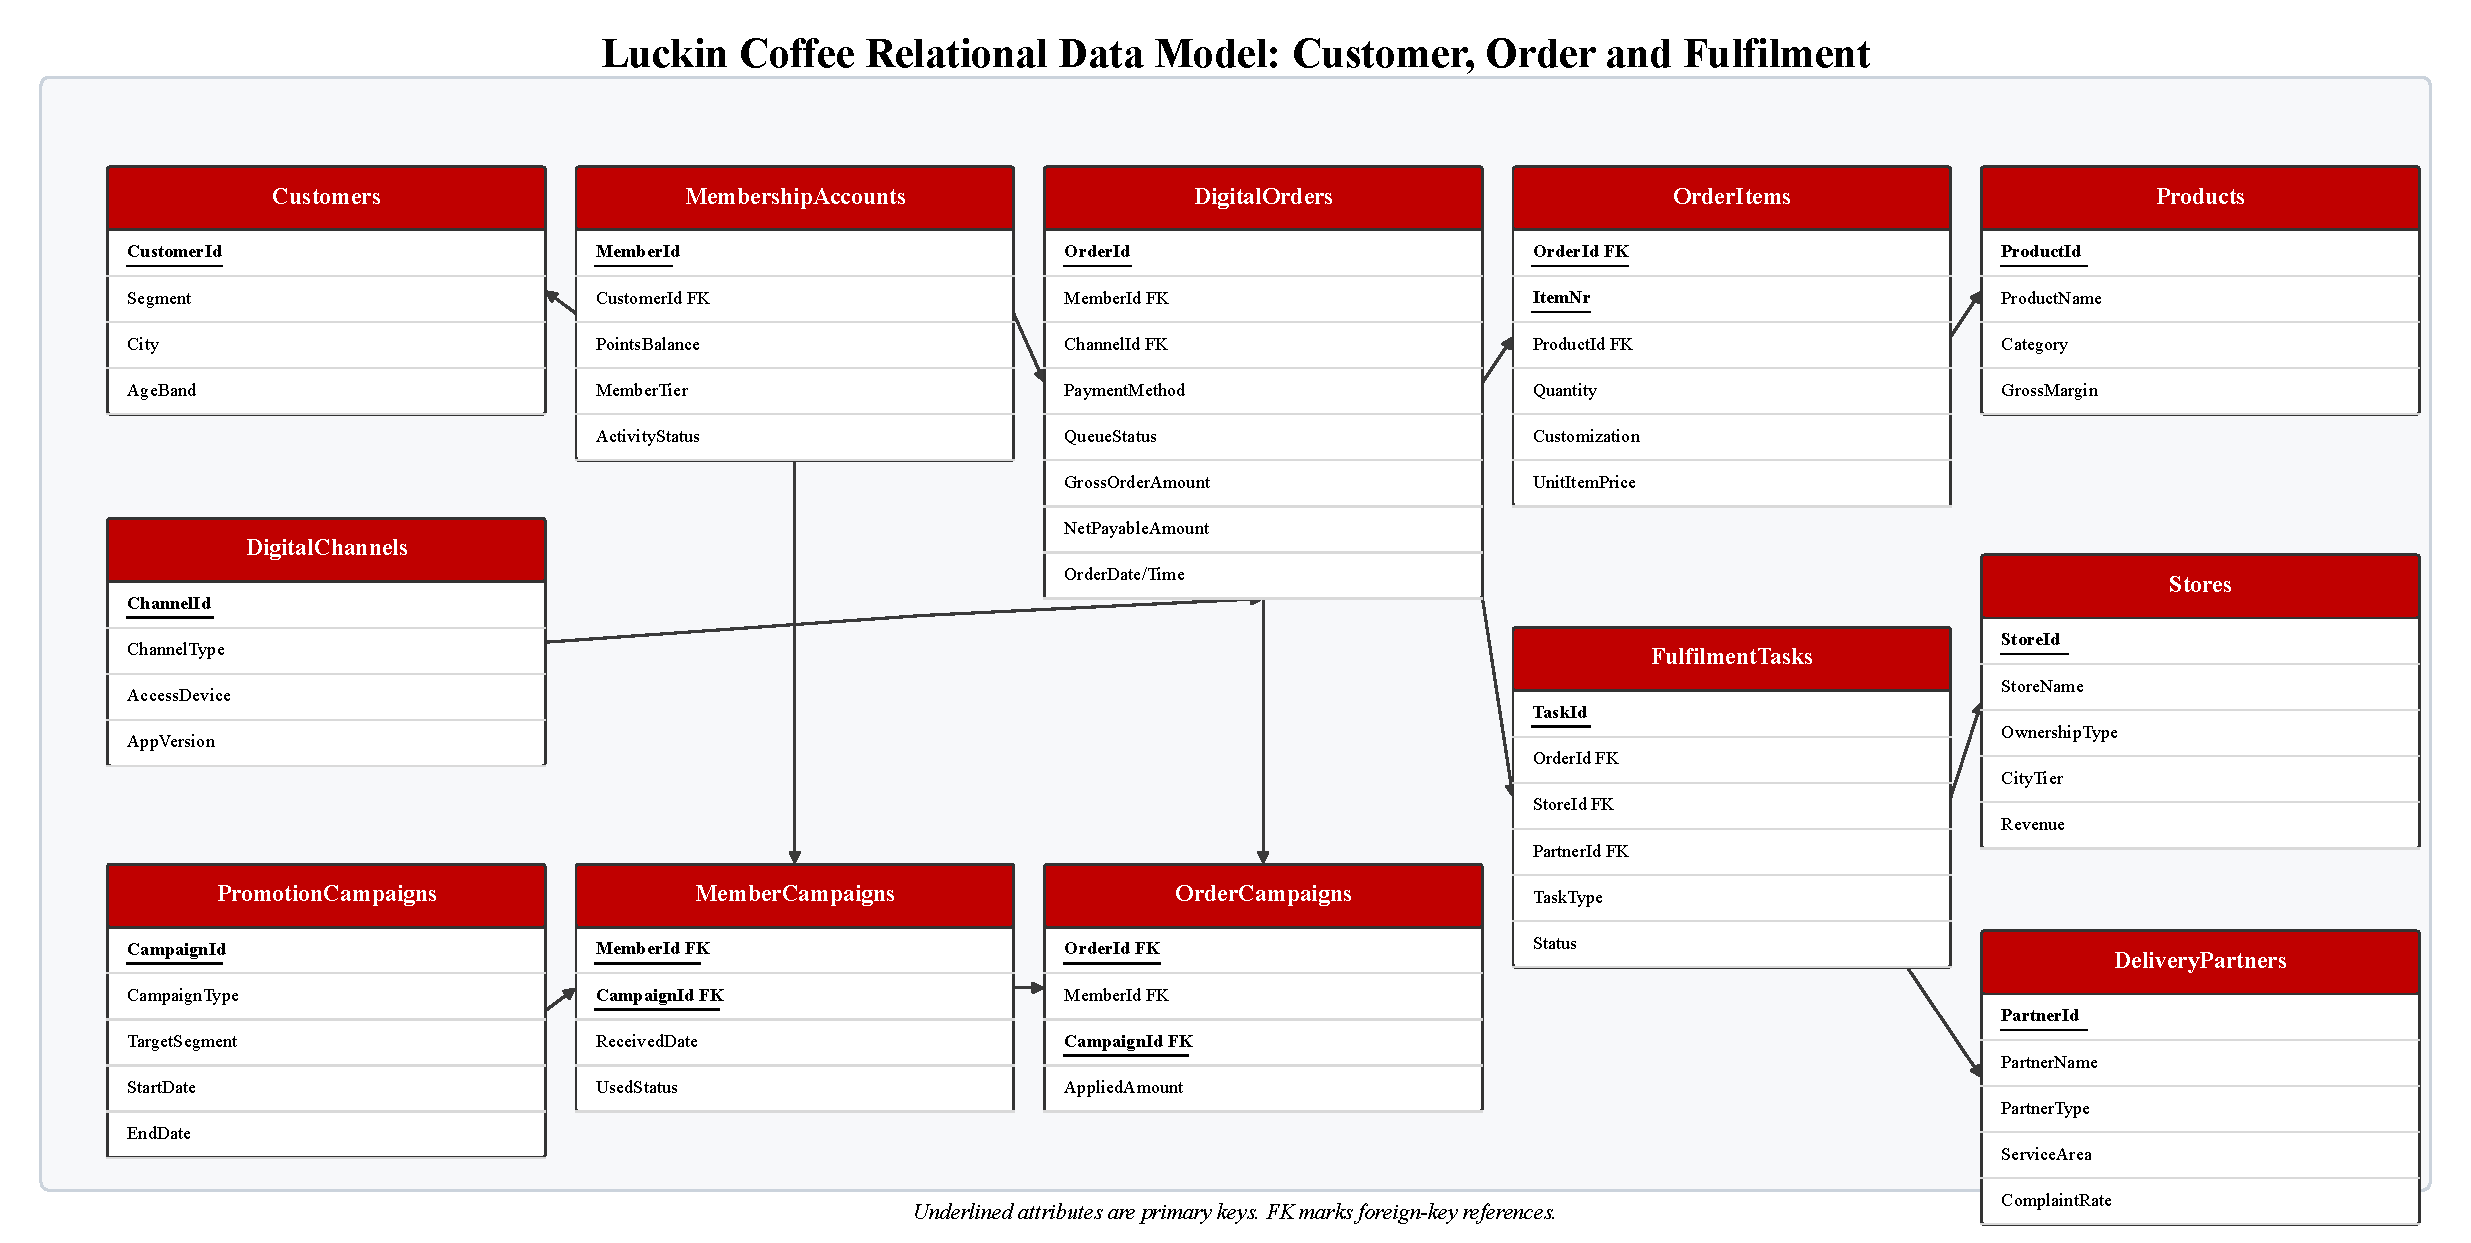
\includegraphics[width=\linewidth,height=16.2cm,keepaspectratio]{schema_operations.pdf}
\vspace{0.2cm}
\caption{Relational data model diagram for customer, order, campaign, and fulfilment relations. Underlined attributes are primary-key attributes; FK marks foreign-key references.}
\end{minipage}
\end{figure}
\end{landscape}
\restoregeometry

\newgeometry{margin=1cm}
\begin{landscape}
\thispagestyle{empty}
\begin{figure}[p]
\centering
\begin{minipage}{26cm}
\centering
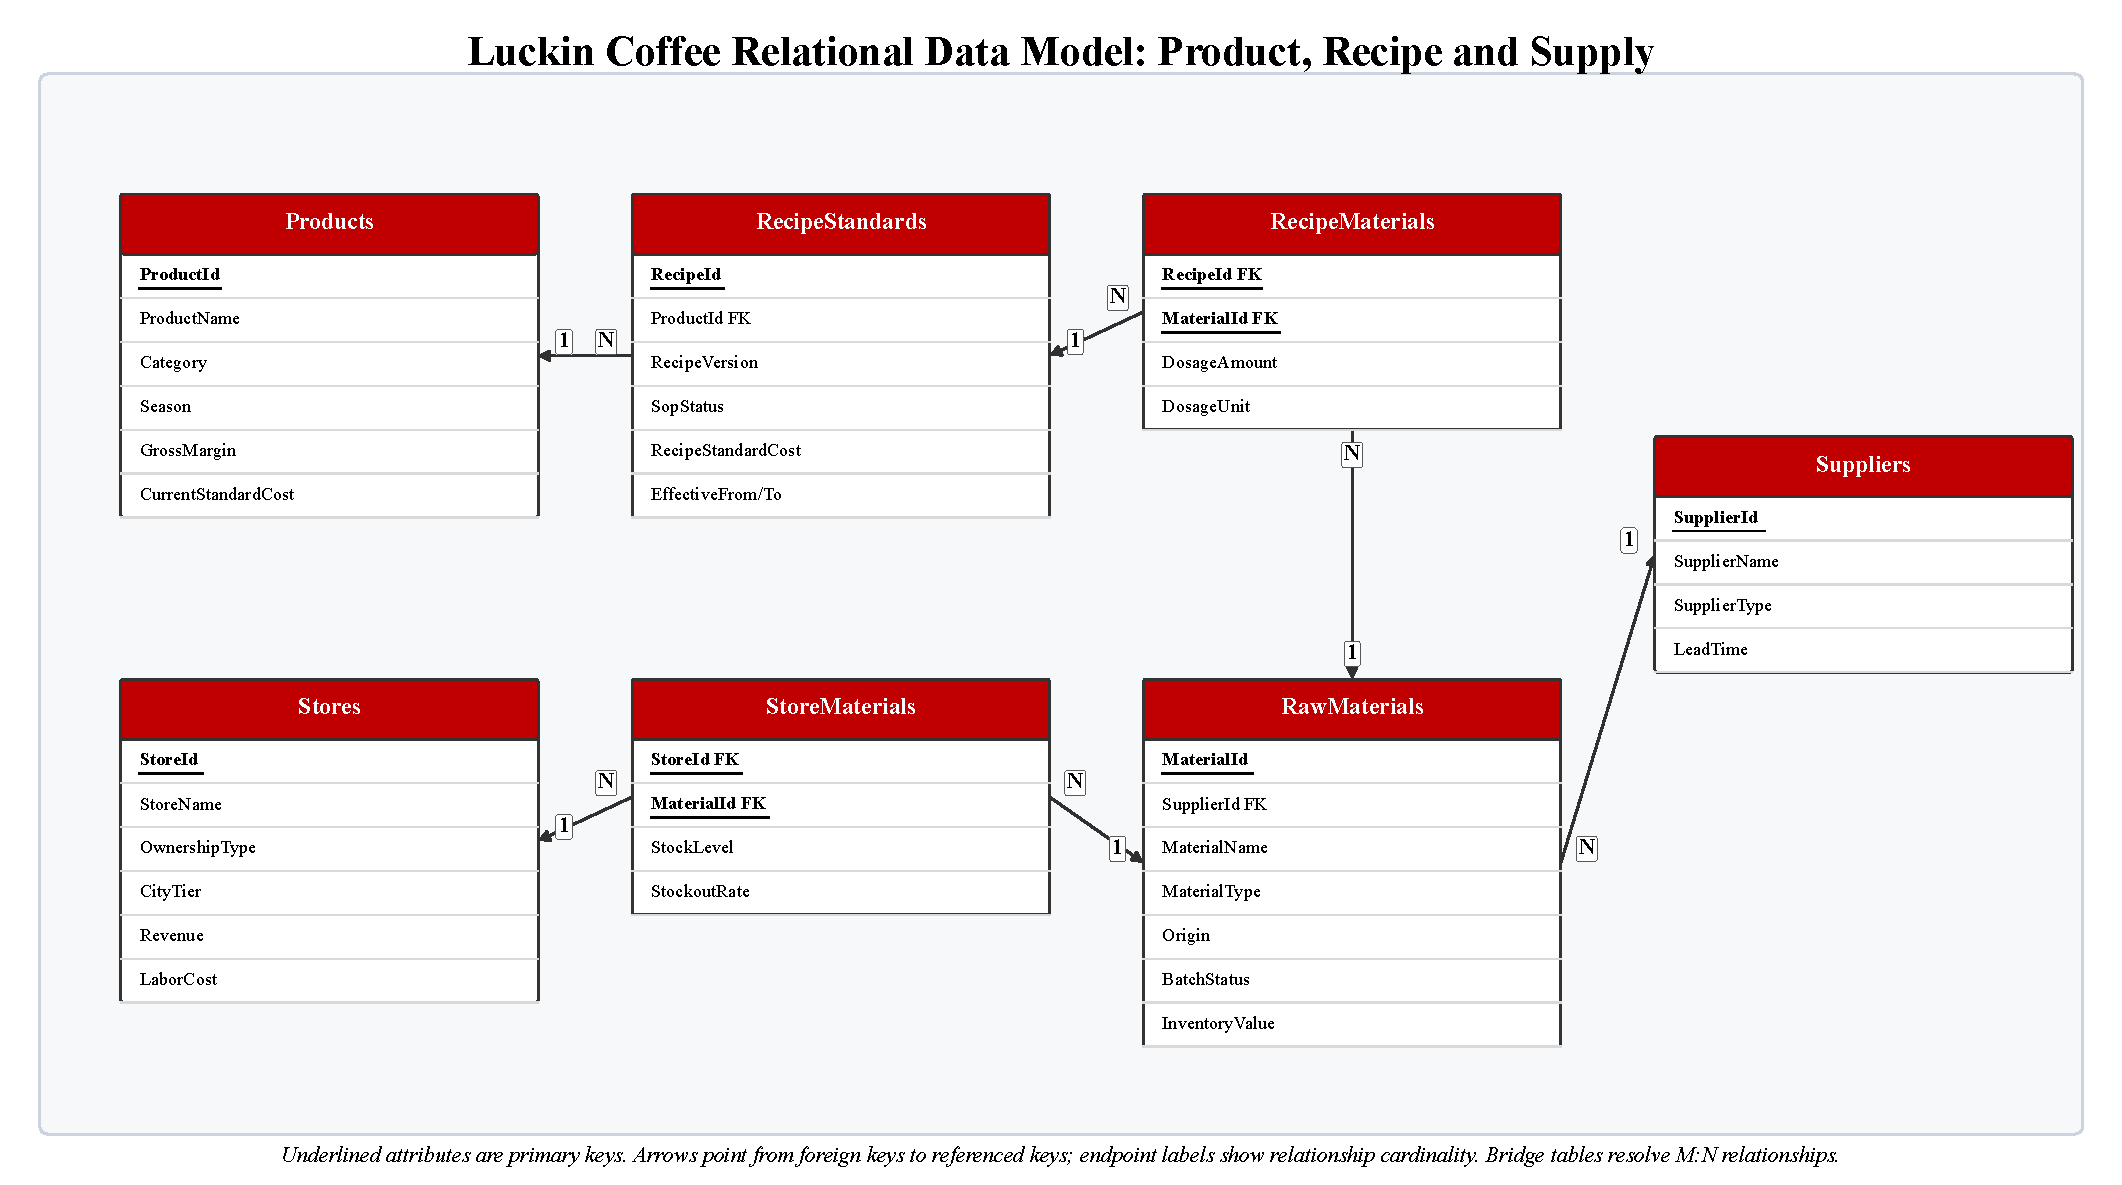
\includegraphics[width=\linewidth,height=16.2cm,keepaspectratio]{schema_supply.pdf}
\vspace{0.2cm}
\caption{Relational data model diagram for product, recipe, material, inventory, and supplier relations. Underlined attributes are primary-key attributes; FK marks foreign-key references.}
\end{minipage}
\end{figure}
\end{landscape}
\restoregeometry

The diagrams are organized around the same business flow as the conceptual model: customer and membership data feed digital orders; orders connect to items, fulfilment tasks, stores, campaigns, and delivery partners; products connect to recipes; recipes and stores connect to raw materials and suppliers.

% =================== IMPLEMENTATION NOTES ===================
\section{Implementation Notes for the Database Schema}

The relational model is implemented in the accompanying SQL schema file. The SQL version uses explicit primary-key, foreign-key, unique, check, and trigger rules so that the database structure preserves the business logic of the conceptual model.

\begin{table}[H]
\centering
\caption{Examples of integrity rules implemented by the schema.}
\small
\begin{tabularx}{\textwidth}{P{4.0cm}Y}
\toprule
\textbf{Rule type} & \textbf{Example in the Luckin Coffee schema} \\
\midrule
Entity integrity & Every base relation has a primary key, such as CustomerId, OrderId, ProductId, StoreId, or MaterialId. \\
Referential integrity & DigitalOrders.MemberId must match an existing MembershipAccounts.MemberId; OrderItems.ProductId must match an existing Products.ProductId. \\
One-to-one control & MembershipAccounts.CustomerId is unique, so one customer cannot have multiple membership account rows in this schema. \\
Bridge-table control & MemberCampaigns, OrderCampaigns, StoreMaterials, and RecipeMaterials use composite primary keys to represent many-to-many relationships. \\
Domain validity & Status and type fields are restricted to allowed values, such as queue status, activity status, task type, ownership type, and batch status. \\
Business arithmetic & NetPayableAmount is constrained to equal GrossOrderAmount minus discounts plus ActualDeliveryFee. \\
Time validity & PromotionCampaigns require StartDate to be earlier than or equal to EndDate; RecipeStandards require a valid effective-date range. \\
Cross-table rule & OrderCampaigns triggers check that a campaign is valid for the order date and that the applied amount does not exceed allowed campaign or order values. \\
\bottomrule
\end{tabularx}
\end{table}

% =================== BUSINESS SCENARIOS ===================
\section{Business Scenarios Supported by the Relational Model}

\subsection{Scenario 1: Mobile Order and Pickup Fulfilment}

When a customer logs in, receives a coupon, submits a coffee order, and picks it up at a store, the database can trace the full chain:
\begin{itemize}[leftmargin=1.3em]
  \item \textbf{Relations joined}: Customers $\rightarrow$ MembershipAccounts $\rightarrow$ MemberCampaigns $\rightarrow$ PromotionCampaigns $\rightarrow$ DigitalOrders $\rightarrow$ OrderCampaigns $\rightarrow$ OrderItems $\rightarrow$ Products $\rightarrow$ FulfilmentTasks $\rightarrow$ Stores.
  \item \textbf{Business value}: The chain shows who bought the drink, which digital channel was used, which coupon was distributed and applied, which product lines were ordered, how long fulfilment took, and which store completed the task.
\end{itemize}

\subsection{Scenario 2: Product Launch and Margin Auditing}

When Luckin launches a new beverage, analysts can evaluate recipe cost, selling price, discounts, and margin performance:
\begin{itemize}[leftmargin=1.3em]
  \item \textbf{Relations joined}: Products $\rightarrow$ RecipeStandards $\rightarrow$ RecipeMaterials $\rightarrow$ RawMaterials $\rightarrow$ Suppliers; Products $\rightarrow$ OrderItems $\rightarrow$ DigitalOrders for actual sales and discounts.
  \item \textbf{Business value}: The chain compares recipe standard cost and ingredient dosage against item revenue and discount behavior, supporting product profitability analysis.
\end{itemize}

\subsection{Scenario 3: Store Inventory Replenishment}

When a store's stock of coffee beans, milk, syrup, or packaging falls below a safety level, the schema supports replenishment decisions:
\begin{itemize}[leftmargin=1.3em]
  \item \textbf{Relations joined}: Stores $\rightarrow$ StoreMaterials $\rightarrow$ RawMaterials $\rightarrow$ Suppliers.
  \item \textbf{Business value}: The system can identify low stock levels by store and material, group replenishment needs by supplier, and connect stockout patterns to store performance.
\end{itemize}

\subsection{Scenario 4: Delivery Reliability Monitoring}

When delivery complaints or waiting time increases, managers can inspect the responsible operational links:
\begin{itemize}[leftmargin=1.3em]
  \item \textbf{Relations joined}: DigitalOrders $\rightarrow$ FulfilmentTasks $\rightarrow$ Stores and DeliveryPartners.
  \item \textbf{Business value}: The schema separates store preparation performance from partner delivery performance, helping managers decide whether the bottleneck is queue preparation, store capacity, or external logistics.
\end{itemize}

% =================== CONCLUSION ===================
\section{Conclusion}

This report completed the two main Seminar 5 tasks for the Luckin Coffee case study. First, the Zachman Framework Row 1 Scope view described the business at a planner level by listing the main data, functions, locations, people, timing concerns, and motivations. This clarified the enterprise boundary before technical design.

Second, the report transformed the Seminar 4 conceptual model into a relational data model. The model contains relations for customers, membership, channels, campaigns, orders, order items, products, recipes, stores, staff, materials, suppliers, fulfilment tasks, and delivery partners. Primary keys, foreign keys, unique constraints, bridge relations, check constraints, and triggers preserve the business relationships identified in the conceptual model. As a result, the schema supports mobile ordering, coupon use, product and recipe management, store fulfilment, inventory replenishment, delivery monitoring, and management reporting.

\begingroup
\small
\setlength{\itemsep}{0pt}
\begin{thebibliography}{9}

\bibitem{zachman1987framework}
Zachman, J. A. (1987).
\emph{A Framework for Information Systems Architecture}.
IBM Systems Journal, 26(3), 276--292.

\bibitem{ylimaeki2005zachman}
Ylimäki, T., \& Halttunen, V. (2005).
\emph{Method engineering in practice: A case of applying the Zachman framework in the context of small enterprise architecture oriented projects}.
Information Knowledge Systems Management, 5(3), 189--209.

\bibitem{sundgren2013egovernance}
Sundgren, B. (2013).
\emph{Methodological and technical perspectives on e-governance}.

\bibitem{elmasri2015db}
Elmasri, R., \& Navathe, S. B. (2015).
\emph{Fundamentals of Database Systems} (7th ed.).
Pearson.

\end{thebibliography}
\endgroup

\end{document}
